\documentclass[main.tex]{subfiles}

\begin{document}
\section{Background}
\subsection{The adiabatic approximation}\label{sec:adiab}
%Kanske ge en full härledning här så småningom, men citera bara Berry tills vidare
%Imagine sitting in a train with a spinning top in somewhat stable movement on the table in
%front of you, see figure \ref{fig:toptrain} for a sketch of the idea. Consider then what would happen were the train to (de)accelerate. If the
%conductor brakes forcefully everything in the cabin experiences a fictitious force in the
%opposite direction of the train acceleration, and the spinning top would fall quickly onto
%the table. If instead the train slows down gradually the fictitious force will be much
%smaller. It can even be small enough in comparison with the properties of the top, its
%angular momentum and distribution of inertia, that the top manages to keep spinning on
%the table. Resilience to perturbation is the very phenomena that keeps a spinning top
%stable in the first place, even if the table were placed in a static house and not a moving
%train. The top keeps its state, the stable position and direction of rotation on the table,
%even though its environment, the train, undergoes change. 
Imagine sitting in a train holding a plate, in which a marble sits at rest much like in
picture \ref{fig:marble}. Consider then what would happen were the train to (de)accelerate.
If the conductor brakes forcefully everything in the cabin experiences a fictitious force
in the opposite direction of the train acceleration. If this force is large enough, the marble would roll up the side
of the rounded plate and fall down to the floor below. If instead the train slows down
gradually the fictitious force will be much smaller, it can even be small enough for the
marble to never roll up the entire height of the plate. Then the marble would stay confined
at the bottom of the porcelain, no matter for how long the train brakes. The marble keeps its
state, the position in the plate, even though its environment, the train, undergoes change.

\begin{figure}[h]
        \centering
        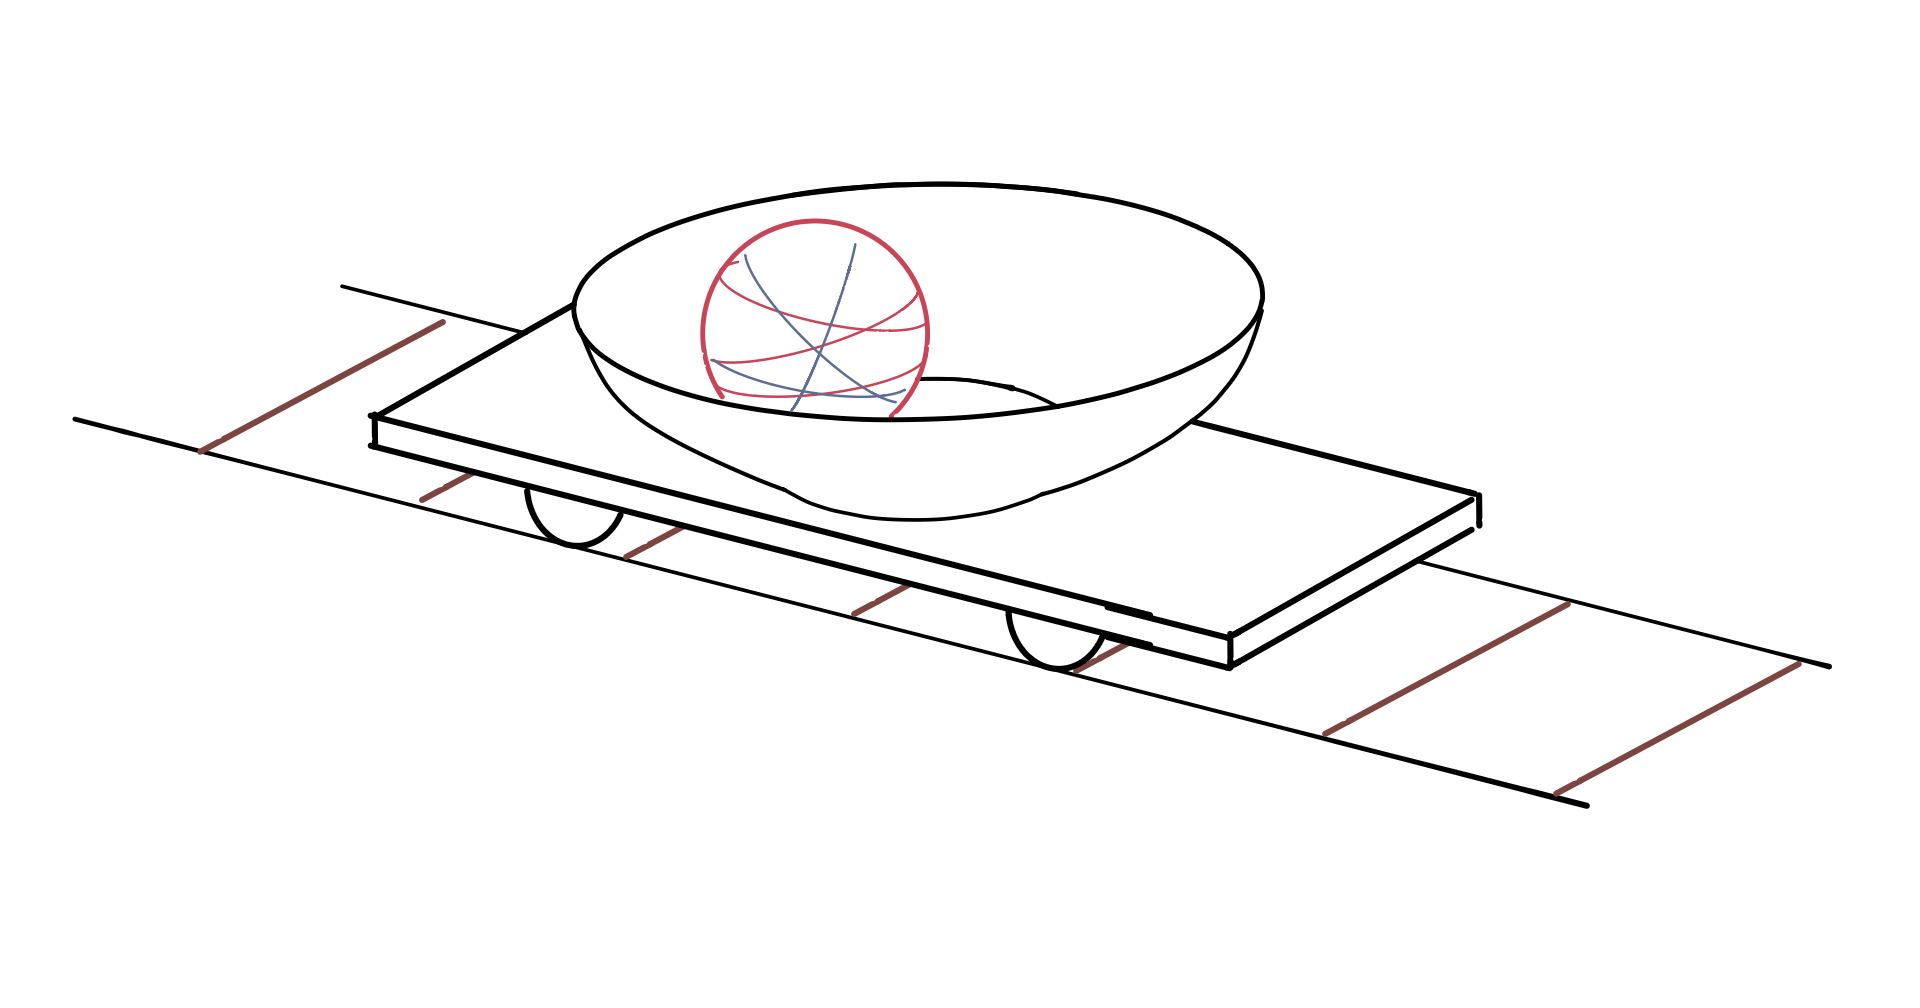
\includegraphics[width=0.8\textwidth]{figures/marble_on_train.png}
        \caption{A marble on a plate on top of a ''train''.}
        \label{fig:marble}
\end{figure}

This thought experiment if translated to the quantum realm, where states are kets or
wavefunctions and the environment is encapsulated in the system Hamiltonian, captures the
essence of the \textit{adiabatic theorem} finalized by Born and Fock \cite{adiab}. Concisely
stated, the original version reads in translation to English:
\begin{displayquote}
A physical system remains in its instantaneous eigenstate if a given perturbation is acting
on it slowly enough and if there is a gap between the eigenvalue and the rest of the
Hamiltonian's spectrum.
\end{displayquote}

In addition to the classical analogue given above, where the speed of the change of
environment was required to be ''slow'', we note an additional requirement on the state: the
energy of the state must not lie close to the energy of any other state available. This
facet will be of great importance in the discussion of geometric phase, and is in a sense the
origin of the synthetic magnetic monopoles. The assumption that the conditions for this
theorem are all satisfied is often referred to as the \textit{adiabatic approximation},
which will be done also in this text.

As an illustrative example consider a particle of spin \(s\) in some external magnetic
field \(\va{B}\). The total energy, and thus Hamiltonian, for such a system is \[
\mathbb{\cal H} = -\gamma \va{B}\cdot \va{S}
.\] 
Here, \(\va{S}\) is the spin operator and \(\gamma\) is a constant determining the magnetic
dipole moment per unit of angular momenta, i.e., it looks typically as \(\gamma =
\frac{g\mu}{\hbar{}}\). Here, \(g\) is a dimensionless \textit{g-factor} and
\(\mu\) is an appropriate magneton. The eigenstates of this Hamiltonian are the same as the
spin eigenstates \(\ket{\va{n}, m}\) in the direction \(\va{n}\) of \(\va{B}\) with the
quantum number \(m\) describing their directional spin eigenvalues. The eigenvalues \(E_m\)
of the
Hamiltonian, the energies of the states, become \[
E_m = -\gamma B \hbar{} m
.\] 
Here \(B\) is the magnetic field strength. The adiabatic theorem states for this
example that any ''slow'' change of the Hamiltonian, that is any slow change of the
magnetic field \(\va{B}\), will not change the quantum number \(m\) of the state occupied
if the system was originally
put into an eigenstate \(\ket{\va{n}, m}\). The only things that change in the state
occupied are
possibly the direction \(\va{n}\) and the energy level \(E_m\). The criterion for the
theorem to hold will here translate into, apart from the speed of change, that \(B\) be
nonzero. If \(B\) were zero the energy levels would be degenerate and the theorem would not be applicable.
\subsection{The geometric phase}\label{sec:geophase}
It was the evolution of systems satisfying the adiabatic theorem that concerned Berry as he
demonstrated the nature of the geometrical phase in the eighties \cite{berry1984}, although non-adiabatic
extensions have been made since \cite{aharonovanandan}. As mentioned in section
\ref{sec:introduction} the adiabatic geometric phase is a contribution to the phase of a
system undergoing adiabatic changes which is \textit{independent} of the energies during the
adiabatic change \cite{erikrev}. %Lite osäker här
Instead it is a contribution dependent only on the path traversed through parameter space,
which in the above example is the three-dimensional space of possible external magnetic
fields. The speed by which the path, often considered to be a loop \(\mathbb{\cal C}\), is traversed matters not for the geometric phase.
Note however that this speed cannot become arbitrarily large, as it would then eventually
break the adiabatic approximation. It is also relevant to the discussion to remind oneself
that the accumulation of phase in quantum mechanics compromises all of dynamics, i.e., all forms
of time evolution can be phrased as changes in the phase of states.

In less abstract terms, it can be shown that an arbitrary quantum energy eigenstate \(\ket{n}\)
(labelled after its energy \(E_n\)) affected by the Hamiltonian \(\mathbb{\cal H}\) will under adiabatic evolution along some loop
\(\mathbb{\cal C}\) accumulate a geometric phase \(\eta_n\). This means that if the loop is
traversed in time \(T\) the state will after one revolution end up as
\(e^{-\frac{i}{\hbar{}}\int_0^T \bra{n}\mathbb{\cal H}\ket{n} dt} e^{i\eta_n}\ket{n}\). Note
the inclusion of the dynamical phase with the first factor, owing to the ''standard'' time
evolution due to energy. The
value of \(\eta_n\) can be calculated from the following
integral \cite{berry1984}:
\begin{align}\label{eq:etaline}
        \eta_n(\mathbb{\cal C}) = i\oint_{\mathbb{\cal C}}
        \bra{n}\ket{\grad_{\va{R}}n}\cdot  d \va{R}
.\end{align}
Here, \(\va{R}\) denotes the parameters at some point in parameter space, so the line integral is
appropriately carried out over that space. Note also that the Hamiltonian and therefore
also all states depend on \(\va{R}\). By Stokes' theorem this integral can be
transformed into a surface integral over any enclosed area in parameter space
\cite{berry1984}. If parameter
space is three dimensional as in the example in section \ref{sec:adiab} above the cross product can additionally be
utilized, and the geometric phase can be recast as:
\begin{align}\label{eq:etasurf}
        \eta_n(\mathbb{\cal C}) = -\iint_{\mathbb{\cal
        C}}d \va{S} \cdot \va{G}_n(\va{R})
,\end{align}
where
\begin{align}\label{eq:synmag}
        \va{G}_n(\va{R}) = \Im \sum_{l \ne n}
        \frac{\bra{n}\grad_{\va{R}}\mathbb{\cal H}\ket{l}\times
                \bra{l}\grad_{\va{R}}\mathbb{\cal H}\ket{n}}{(E_l -
                        E_n)^{2}}
.\end{align}

It is here that the monopole field makes its entrance. While the integrand of equation
\ref{eq:etaline} is only defined up to the gradient of an arbitrary differentiable function, owing to an arbitrary phase factor of
the eigenstate basis, the field \(\va{G}_n\) is but the curl of this integrand and thus
independent of this arbitrary term. The phase evolution due to the geometric phase has
then taken the form of the time evolution through a magnetic field \(\va{G}_n\) derived
from the vector potential
\begin{align}\label{eq:Dfield}
        \va{D}_n = i\bra{n}\grad_{\va{R}}\ket{n}
.\end{align}
We call \(\va{G}_n\) the synthetic magnetic field, or the synthetic gauge field, and consider
it the field the action of which results in the geometric phase. The monopole
structure so often mentioned previously is present in precisely this field, by which it is
meant that the singularities of this field which occur at points of energy degeneration may
infer a non-zero divergence \(\div \va{G}_n\). Since the field is not defined at these points, divergence
should here be interpreted in the rather loose sense of a closed flux integral about some
point divided by the enclosed volume. A nonzero divergence of a magnetic field is not allowed for
standard Maxwellian magnetic fields and would imply some form of magnetic charge or
monopole. Even though our synthetic field does not follow Maxwell's equations it shares
the magnetic field property of being the curl of a vector potential, and as will be clear
in section \ref{sec:BOinterp} also magnetic properties in how it establishes dynamics. For
these reasons the monopoles present at the degeneracies allow us to study, in a sense, the
action of Maxwellian magnetic monopoles. It may be worthwhile to emphasize that the
singular nature of the field at the energy degeneracies, that the field is there undefined,
is crucial to the nonzero divergence. This mimics the model of electrical point charges,
but also makes the dependence on the adiabatic approximation abundantly clear.
\subsection{Regarding the monopoles}\label{sec:regmono}
The system outlined in the final paragraph of section \ref{sec:adiab} forms a sort of minimal working example of a
synthetic field. The energies of different states are there degenerate only for an
external magnetic field of zero magnitude, that is at the origin of parameter space, so the
synthetic field has a monopole precisely at the origin. The action from the synthetic
field, that is the accumulation of geometrical phase, could be achieved either from slowly
varying the external field magnitude and direction or likewise from the slow movement of the
particle through an inhomogeneous external field yielding the same effect. It is further
the case for this simple example that the synthetic field not only contains monopoles, but
that it is \textit{purely} monopolar in origin. This is to say that a ''charge'' placed at
the origin emanating a spherically symmetric field that falls off as the inverse square of the distance yields
precisely the synthetic field in question, the field is only due to
''charges'' \cite{berry1984}. It is important to note that this must not
always be the case, the synthetic magnetic field may, depending on the Hamiltonian, take a
form which is not possible to describe only through inverse-square falloff from 
charges. It could even be the case that no such charges are present at all, what the
synthetic field simply does is to allow for them. %%Tror jag stämmer? Dubbelkolla med Erik
%Någon kommentar om "mest generella fältet/inga restriktioner?

One case for which the synthetic field is \textit{not} purely monopolar is two spin
constituents interacting with both an external magnetic field and each other as shown by Eriksson and Sjöqvist
\cite{eriksson}, much like the system outlined in section \ref{sec:aselsys}. These authors further note that the nonzero curl of a synthetic field that is not purely
monopolar can be used to extend the allegory between synthetic and Maxwellian 
fields through a synthetic electrical ''current'' defined through the curl of the synthetic
magnetic field. The main
effect of spin-spin interaction of composite spin systems is however the ''splitting'' or
movement of magnetic charge away from the origin of parameter space yielding more exotic fields. This movement of magnetic monopoles is continuous
with respect to the spin-spin interaction parameters, and will be fully determined by these
parameters. It is further important to the splitting of monopoles that the spin-spin interaction is of
such nature that the total system is not spherically symmetric. Were the system spherically
symmetric, the synthetic field would have to be likewise in parameter space, and any
monopoles would be restricted to sit at the origin. Since the system outlined in section
\ref{sec:aselsys} contains precisely an Ising interaction along some selected axis the
synthetic field is in this case not fully spherically symmetric, but must have a rotational symmetry
determined by said axis. 

For the sake of this body of work we note that the synthetic field of the dumbbell
model will be nontrivial
in nature, carries distinct synthetic monopoles and further may exhibit nonzero curl, so
that it is not purely monopolar.
\end{document}

